\section{Architecture}

Figure \ref{fig:arch_01} illustrates a high level overview of the distributed audio proessing environment. The user of the system interacts with the audio production software running on the host CPU and can choose to activate an audio processing plugin on a specific audio track. A single audio plugin might contain one or several individual processors. Processor that are enabled for distributed processing will search for a corresponding processor on a network SBC device.

The devices are networked via gigabit ethernet. It is assumed that the network is not being used for any other significant traffic.

\begin{figure}[H]
    \centering
    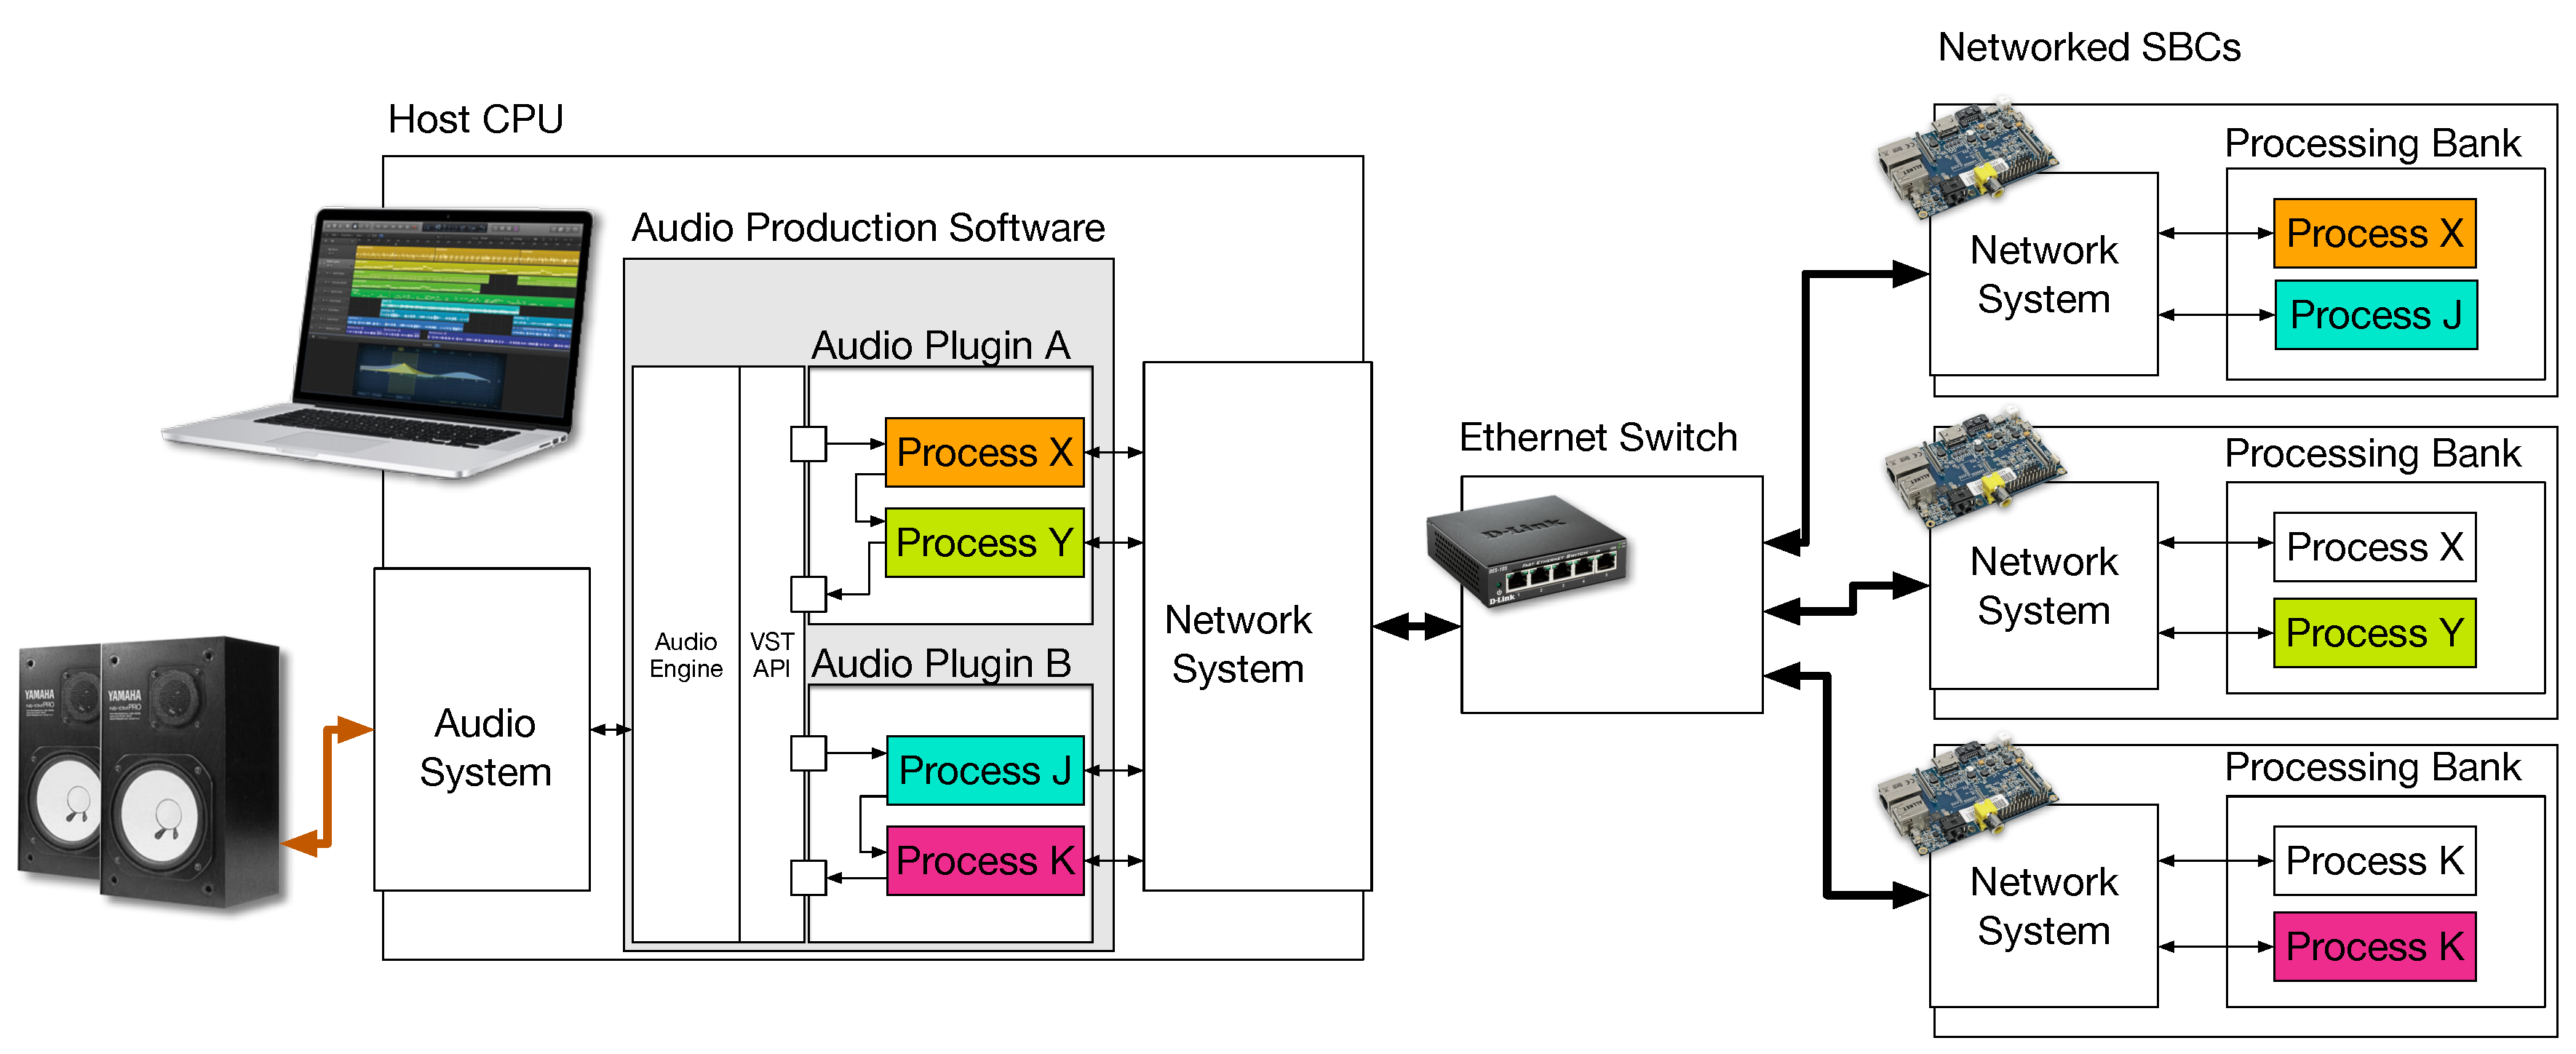
\includegraphics[width=\textwidth]{assets/architecture_01.pdf}
    \caption{Architectural Overview}
    \label{fig:arch_01}
\end{figure}

Figure \ref{fig:arch_02} zooms in on the components involved in realtime audio on the CPU. The audio hardware needs to provide a constant stream of data to it's digital to analog converters. It does this by periodically polling the operating system for a buffer of data via hardware interrupts. The requested buffer size can be as small as 32 samples and the polling intervals less than 1 ms depending on the hardware and drivers.

The operating system provides an abstraction layer in the form of an API to the application software. This gives the application software a single API to interface with regardless of the brand of audio hardware and drivers installed.

The VST API is another abstraction layer that offers a unified interface for plugin vendors to develop against. But VST is not the only plugin API. The Juce library offers it's own plugin API to develop against, which is simpler and abstracts away the differences between other plugin APIs.

\begin{figure}[H]
    \centering
    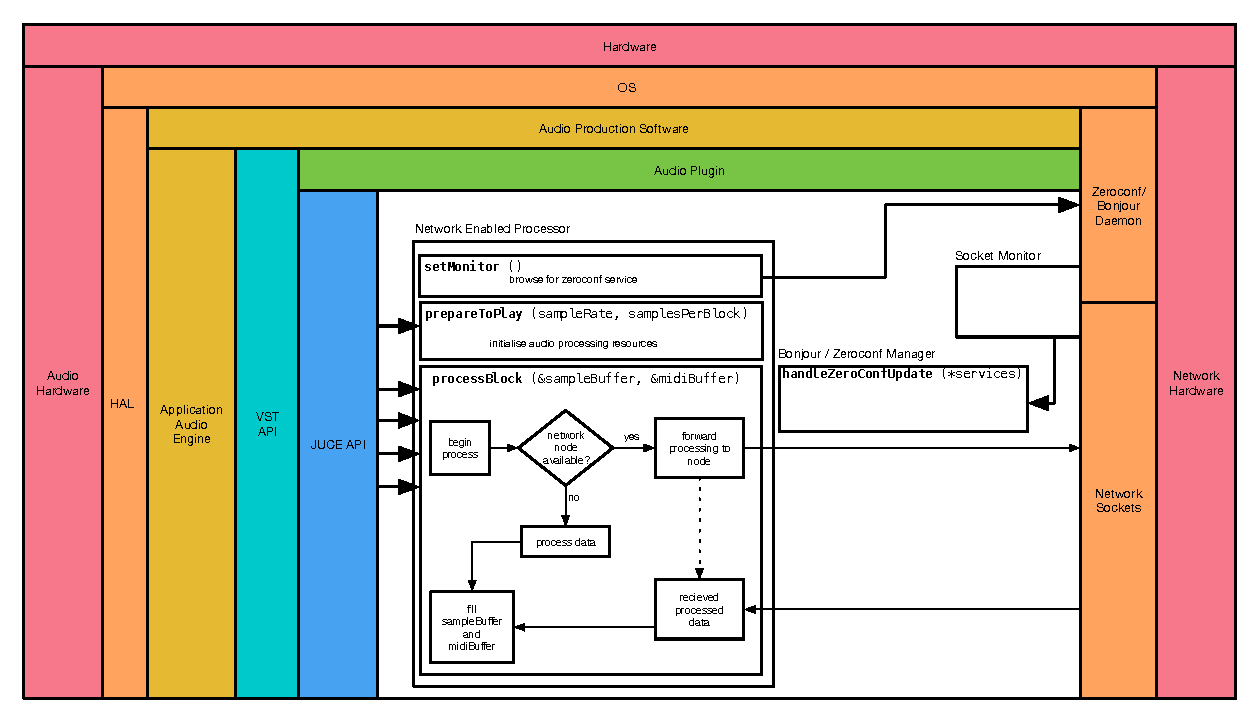
\includegraphics[width=\textwidth]{assets/architecture_02.pdf}
    \caption{Host CPU Overview}
    \label{fig:arch_02}
\end{figure}
